%!Tex Program = xelatex
\documentclass[a4paper]{article}
\usepackage{fontspec, xunicode, xltxtra}
\usepackage[slantfont,boldfont]{xeCJK} % 允许斜体和粗体
\usepackage{geometry}
\usepackage{indentfirst}
\usepackage{lastpage}
\usepackage{multirow}
\usepackage{multicol}
\usepackage{titlesec}
\usepackage{enumerate}
\usepackage{booktabs}
\usepackage{extarrows}
\usepackage{fancyhdr,fancybox}
\usepackage[table]{xcolor}
\usepackage{float}
\usepackage{tikz}
%\usepackage{amssymb}
%\usepackage{amsmath}
%\usepackage{caption}
%\usepackage{dirtree}
%\usepackage{algorithm}
%\usepackage{algpseudocode}
\usepackage{listings}
\usepackage[colorlinks,linkcolor=black]{hyperref}

\geometry{left=2.5cm,right=2.5cm,top=2.5cm,bottom=2.5cm}

%cmd “fc-list :lang=zh-cn”
\defaultfontfeatures{Mapping=tex-text}
\setmainfont{Book Antiqua}   % 英文衬线字体 Times New Roman, Palatino Linotype
\setmonofont{Consolas}   % 英文等宽字体 Monaco
\setsansfont{Consolas} % 英文无衬线字体 Arial, Futura, Optima
\setCJKmainfont{SimSun}   % 设置缺省中文字体
\setCJKmonofont{FangSong}   % 设置等宽字体
\setCJKsansfont{SimHei}   % 设置无衬线字体 Microsoft YaHei

\newfontfamily\timesroman{Times New Roman}
\newfontfamily\consolas{Consolas}

\newfontfamily\ensong{SimSun}
\newfontfamily\enhei{SimHei}
\newfontfamily\enyahei{Microsoft YaHei}
\newfontfamily\palatino{Palatino Linotype}
\newfontfamily\nimbus{Nimbus Sans L}
\newfontfamily\enkai{STKaiti}
\newfontfamily\enfangsong{FangSong}
\newfontfamily\akaDora[Path=../]{akaDora.ttf}

\setCJKfamilyfont{song}{SimSun}
\newcommand{\song}{\CJKfamily{song}\ensong}
\setCJKfamilyfont{heiti}{SimHei}
\newcommand{\heiti}{\CJKfamily{heiti}\enhei}
\setCJKfamilyfont{yahei}{Microsoft YaHei}
\newcommand{\yahei}{\CJKfamily{yahei}\enyahei}
\setCJKfamilyfont{kaiti}{STKaiti}
\newcommand{\kaiti}{\CJKfamily{kaiti}\enkai}
\setCJKfamilyfont{fangsong}{FangSong}
\newcommand{\fangsong}{\CJKfamily{fangsong}\enfangsong}

\XeTeXlinebreaklocale "zh"
\XeTeXlinebreakskip = 0pt plus 1pt minus 0.1pt

\titlespacing*{\chapter} {0pt}{50pt}{40pt}
\titlespacing*{\section} {0pt}{3.5ex plus 1ex minus .2ex}{2.3ex plus .2ex}
\titlespacing*{\subsection} {0pt}{3.25ex plus 1ex minus .2ex}{1.5ex plus .2ex}
\titlespacing*{\subsubsection}{0pt}{3.25ex plus 1ex minus .2ex}{1.5ex plus .2ex}
\titlespacing*{\paragraph} {0pt}{3.25ex plus 1ex minus .2ex}{1em}
\titlespacing*{\subparagraph} {\parindent}{3.25ex plus 1ex minus .2ex}{1em}

\titleformat{\section}{\Large \bf \nimbus}{\thesection}{1em}{}
\titleformat{\subsection}{\large \bf \nimbus}{\thesubsection}{0.5em}{}

\setlength{\parskip}{0.5\baselineskip}
\setlength{\abovedisplayskip}{1pt}
\setlength{\belowdisplayskip}{1pt}

\usetikzlibrary{arrows,positioning}
\newcommand\nbvspace[1][3]{\vspace*{\stretch{#1}}}
\newcommand\nbstretchyspace{\spaceskip0.5em plus 0.25em minus 0.25em}
\newcommand{\nbtitlestretch}{\spaceskip0.6em}

\pagestyle{fancy}


\lstset{
    basicstyle=\small,
    backgroundcolor=\color{white},
    %keywordstyle=\color{keywordcolor}\bfseries, %\underbar,
    keywordstyle=\color{blue}\bfseries,
    %morekeywords={*,keyword_a,keyword_b},
    sensitive=true,
    identifierstyle=\small,
    showspaces=false,
    showstringspaces=false,
    showtabs=false,
    tabsize=4,
    frame=single,
    commentstyle=\color{olive} \textit,
    stringstyle=\ttfamily,
    showstringspaces=false,
    captionpos=b,
    breaklines=true,
    breakatwhitespace=true,
  }

\lstdefinelanguage{Makefile} {
  numberblanklines=false,
  keywordstyle=\color{blue}\bfseries,
  morekeywords={gedit,ls,rm,source,sudo,tar},
}

\lstdefinelanguage{LinuxTerminal} {
  numberblanklines=false,
  keywordstyle=\color{blue}\bfseries,
  morekeywords={cat,cd,chmod,gedit,ln,ls,
    make,mkdir,rm,source,sudo,tar,touch},
  morecomment=[l]{\#},
}

\lstdefinelanguage{PlainText} {
  numberblanklines=false,
}



\usepackage{tikz}

\begin{document}
  \thispagestyle{empty}
  \begin{center}
    \bfseries
    \nbvspace[2]
    \begin{figure}[H]
      \centering
      
\includegraphics[width=0.6\textwidth]{../logo.pdf}
    \end{figure}
    {\Huge GDPLS Movie} \\[10pt]
    {\LARGE\akaDora Grand Duke of Programming Language Script}\\[10pt]
    {\Huge 2017 June} \\
    \nbvspace[1]
    \Huge Sprint Plan\\
    \nbvspace[1]
    \normalsize Generated \& Compiled By \XeLaTeX
    \nbvspace[3]
  \end{center}
  \newpage

  \lhead{\emph{VISION TABLE}}
  \begin{table}[H]
    \centering
    \renewcommand\arraystretch{1.3}
    \rowcolors{2}{blue!50}{blue!20}
    \begin{tabular}{lllp{28em}}
      %\rowcolors{1}{blue!80}{blue!10}
      \multicolumn{4}{c}{\heiti 版本日志}\\
      版本号 & 修改人 & 修改时间 & \multicolumn{1}{c}{说明} \\
      1.0.0 & 方铭 & 2017.4.8 & 设计初稿\\
      &&&\\
      &&&\\ % span text width
    \end{tabular}
  \end{table}
  \newpage
  \lhead{}
  {\Huge \bf \underline{BetaGO,sprint 1}}
  
  \par {\bf Sprint Goal}
  \begin{itemize}
    \item 实现座位评价的相关功能
    \item 实现座位推荐功能
  \end{itemize}
  
  \par {\bf Sprint Backlog (estimates in parenthesis)}
  \begin{itemize}
    \item 网站基本框架搭建(10)
    \item 查看座位评价(2)
    \item 发表座位评价(2)
    \item 座位推荐(3)
  \end{itemize}


  \par {\bf Sprint Backlog (estimates in parenthesis)}
  \begin{itemize}
    \item 网站基本框架搭建(10)
    \item 查看座位评价(2)
    \item 发表座位评价(2)
    \item 座位推荐(3)
  \end{itemize}
\indent Estimated velocity: 17

\par {\bf Schedule}
  \begin{itemize}
    \item Sprint period: 2017-04-03 to 2017-04-10
    \item Daily scrum: 22:00 – 22:15, at sac
    \item Sprint demo: 2017-04-10, 22:00, at sac
  \end{itemize}

\par {\bf Team}
  \begin{itemize}
    \item 徐佳豪
    \item 陈锐煌
    \item 卢卓君
    \item 徐广晖
    \item 郑斯达
    \item 方铭
  \end{itemize}

\newpage
\section{Detailed Sprint Backlog}
\begin{table}[H]
  \centering
  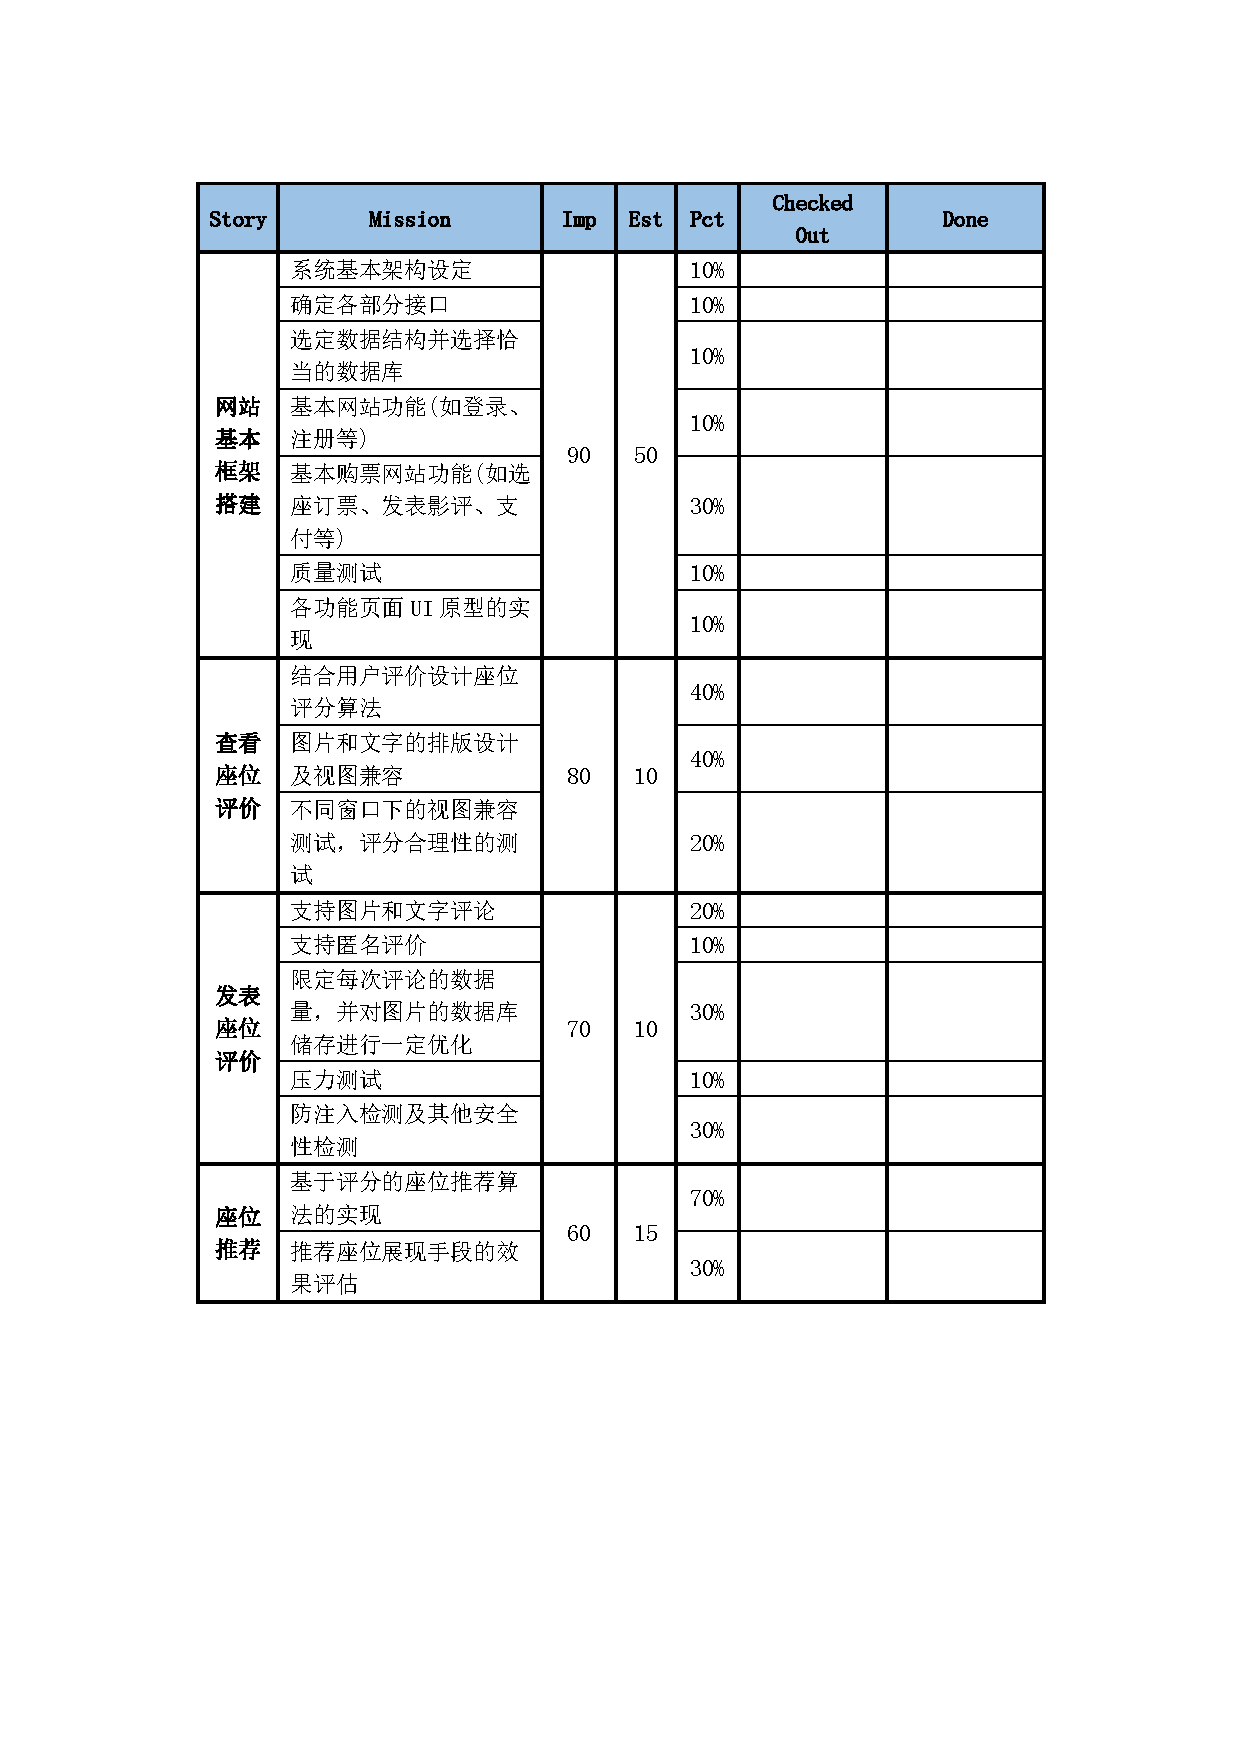
\includegraphics[width=\textwidth]{table.pdf}
\end{table}

\section{字段说明}
\begin{table}[H]
  \centering
  \begin{tabular}{lp{35em}}
    Story & 故事 \\
    Mission & 由故事划分成的多个子任务 \\
    Imp & 重要性评估数值。分数越高越重要。 \\
    Est & 团队的初步实现估算,表示与其他故事相比,完成该故事所需的工作量。单位为一个“理想的人天(man-day)”。 \\
    Pct & 该子任务的工作量占其所在故事工作量的比例。 \\
    Checked Out & 当前正在实现该任务的人。 \\
    Done & 该任务是否完成。 \\
  \end{tabular}
\end{table}
%\begin{description}
%  \item[Story] \indent 故事。
%  \item[Mission] \indent 由故事划分成的多个子任务。
%  \item[Imp] \indent 重要性评估数值。分数越高越重要。
%  \item[Est] \indent 团队的初步实现估算,表示与其他故事相比,完成该故事所需的工作量。单位为一个“理想的人天(man-day)”。
%  \item[Pct] \indent 该子任务的工作量占其所在故事工作量的比例。
%  \item[Checked Out] \indent 当前正在实现该任务的人。
%  \item[Done ] \indent 该任务是否完成。
%\end{description}



\end{document}
